\documentclass{webofc}

\usepackage{graphicx}
\usepackage{tabularx}
%\usepackage{cite}
\usepackage{subcaption}
\captionsetup[figure]{labelsep=period,labelfont=bf}
\captionsetup[table]{labelsep=period,labelfont=bf}

% Set serif font to Paratype
%\usepackage{paratype}
\usepackage[varg]{txfonts}
\usepackage[T1]{fontenc}

% Colours

\usepackage{xcolor}      % Colours
\usepackage{colortbl}    % Colour tables

% CERN blue is Pantone 286 = RGB 56 97 170, defined as cern@blue below
\definecolor{cern@ltblue}{rgb}{0.415686,0.611765,0.964706} % RGB 106 156 246
\definecolor{cern@blue}  {rgb}{0.219608,0.380392,0.666667} % RGB  56  97 170
\definecolor{cern@dkblue}{rgb}{0.082353,0.184314,0.364706} % RGB  21  47  93

% Complimentary colours
\definecolor{cern@ltcomp}{rgb}{0.666667,0.525490,0.219608} % RGB 170 134  56
\definecolor{cern@dkcomp}{rgb}{0.364706,0.266667,0.047059} % RGB  93  68  12

% Hyperlinks
\usepackage{hyperref}
\hypersetup{
  colorlinks=true,
  citecolor=cern@blue,
  linkcolor=cern@dkblue,
  urlcolor=cern@ltblue,
  unicode=true
}

% SI Units (computer science style)
\usepackage[binary-units=true, per-mode=symbol]{siunitx}

% Figures layout
\usepackage{wrapfig}
\usepackage{subcaption}

\begin{document}
\title{\raggedright CERN Tape Archive: production status, migration from CASTOR and new features}
\author{Eric Cano\inst{1}\fnsep\thanks{\email{{eric.cano, vladimir.bahyl, cedric.caffy, german.cancio.melia, michael.davis, julien.leduc, steven.murray}@cern.ch}}
   \and Vladim\'ir Bahyl\inst{1}\fnsep\footnotemark[1]
   \and C\'edric Caffy\inst{1}\fnsep\footnotemark[1]
   \and Germ\'an Cancio\inst{1}\fnsep\footnotemark[1]
   \and Michael Davis\inst{1}\fnsep\footnotemark[1]
   \and Viktor Kotlyar\inst{2}\fnsep\thanks{\email{viktor.kotliar@ihep.ru}}
   \and Julien Leduc\inst{1}\fnsep\footnotemark[1]
   \and Tao Lin\inst{3}\fnsep\thanks{\email{lintao@ihep.ac.cn}}
   \and Steven Murray\inst{1}\fnsep\footnotemark[1]
   }
\institute{\inst{}{CERN---European Organization for Nuclear Research, 1211 Geneva 23, Switzerland} \and
           \inst{}{Institute for High Energy Physics named by A.A. Logunov of National
                   Research Center ``Kurchatov Institute'', Nauki Square 1, Protvino, Moscow
                   region, Russia, 142281} \and
           \inst{}{Institute of High Energy Physics, Chinese Academy of Sciences}}

\abstract{
During 2019 and 2020, the CERN tape archive (CTA) will receive new data from LHC experiments and import
existing data from CASTOR, which will be phased out for LHC experiments before Run 3.

\hspace{1.5em}This contribution will present the statuses of CTA as a service and of its integration with
EOS and FTS and the data flow chains of LHC experiments.

\hspace{1.5em}The latest enhancements and additions to the software as well as the development outlook will be presented.
With the development of the repack function, a necessary behind-the-scenes feature, CTA can now take over
custodial data and handle media migration, compaction and failures. Further metadata handling optimisations
allowed doubling the maximum file rate performance to 200Hz per queue.

\hspace{1.5em}New retrieve scheduling options are being developed at the request of experiments, with optional
FIFO behaviour to ensure better control of the timing for datasets retrieve, and fair share support for competing
activities within the same VO.

\hspace{1.5em}Support for multiple backend databases (Oracle, PostgreSQL, MySQL) have been developed at CERN
and contributed by external institutes.

\hspace{1.5em}This contribution will also report on the challenges of and solutions for migrating data from
the decades old CASTOR to CTA. The practical example of the preparation for the migration of ATLAS data will be presented.}

\maketitle

\section{Introduction}
\label{introduction}
The LHC particle accelerator at CERN will undergo upgrades for the upcoming run 3 (2021-2024) and the high luminosity run 4 (starting 2027).
As a consequence, the High Energy Physics experiments at the LHC expect to largely exceed \cite{atlas_future_chep2018} the exponential growth trends that the storage industry has followed in 
data volume per unit cost~\cite{Insic_roadmap_2019} and has so far allowed the fulfilment of their storage requirements on a flat budget.

In anticipation of this storage challenge, the experiments are trying to optimise their usage of resources. For example, the concept of a data carousel is
currently being explored by the ATLAS experiment~\cite{atlas_data_carousel_update_2018}.

The CERN Tape Archive (CTA) is a replacement for and evolution from its predecessor, CASTOR~\cite{castor2007}. While CASTOR provides tape
storage, a disk cache and staging functionality, the goal of CTA is simply to provide tape backend to EOS~\cite{Peters_2011}, the low latency
disk storage system used at CERN T0 for DAQ and analysis.

Pre-production deployments of EOSCTA have been provided to experiments, delivering first performance measurements. Those tests also allowed the validation
of the integration with some experiments' offline frameworks.

New features have also been introduced and will be discussed in the following sections.


%The High Energy Physics experiments at CERN generate a deluge of data which must be efficiently archived
%for later retrieval and analysis. The CERN Tape Archive (CTA) is the new tape storage system for the custodial
%copy of the physics data.
%
%CTA is a replacement for and evolution from its predecessor, CASTOR~\cite{castor2007}. While CASTOR provides tape
%storage, a disk cache and staging functionality, CTA has a more simple design philosophy.
%CTA is implemented as the tape back-end to the EOS disk system~\cite{eos_chep2015}, and all disk cache functions
%are delegated to EOS. As EOS is already the \textit{de facto} storage system for physics analysis at CERN,
%CTA aims to provide the ``best of both worlds''---EOS disk and CASTOR tape.
%
%The main goal of CTA is to make more efficient use of the tape drives, to handle the higher data rates
%anticipated during Run--3 and Run--4 of the Large Hadron Collider (LHC). In our previous paper~\cite{cta_chep2016},
%we described how this was to be achieved, by introducing a pre-emptive drive scheduler which can keep tape drives
%running at full speed all of the time.

\section{CTA service, integration with EOS and FTS}
\subsection{The CTA deployment model}
%\subsubsection{Deployment model}

\begin{wrapfigure}{L}{0.55\textwidth}
   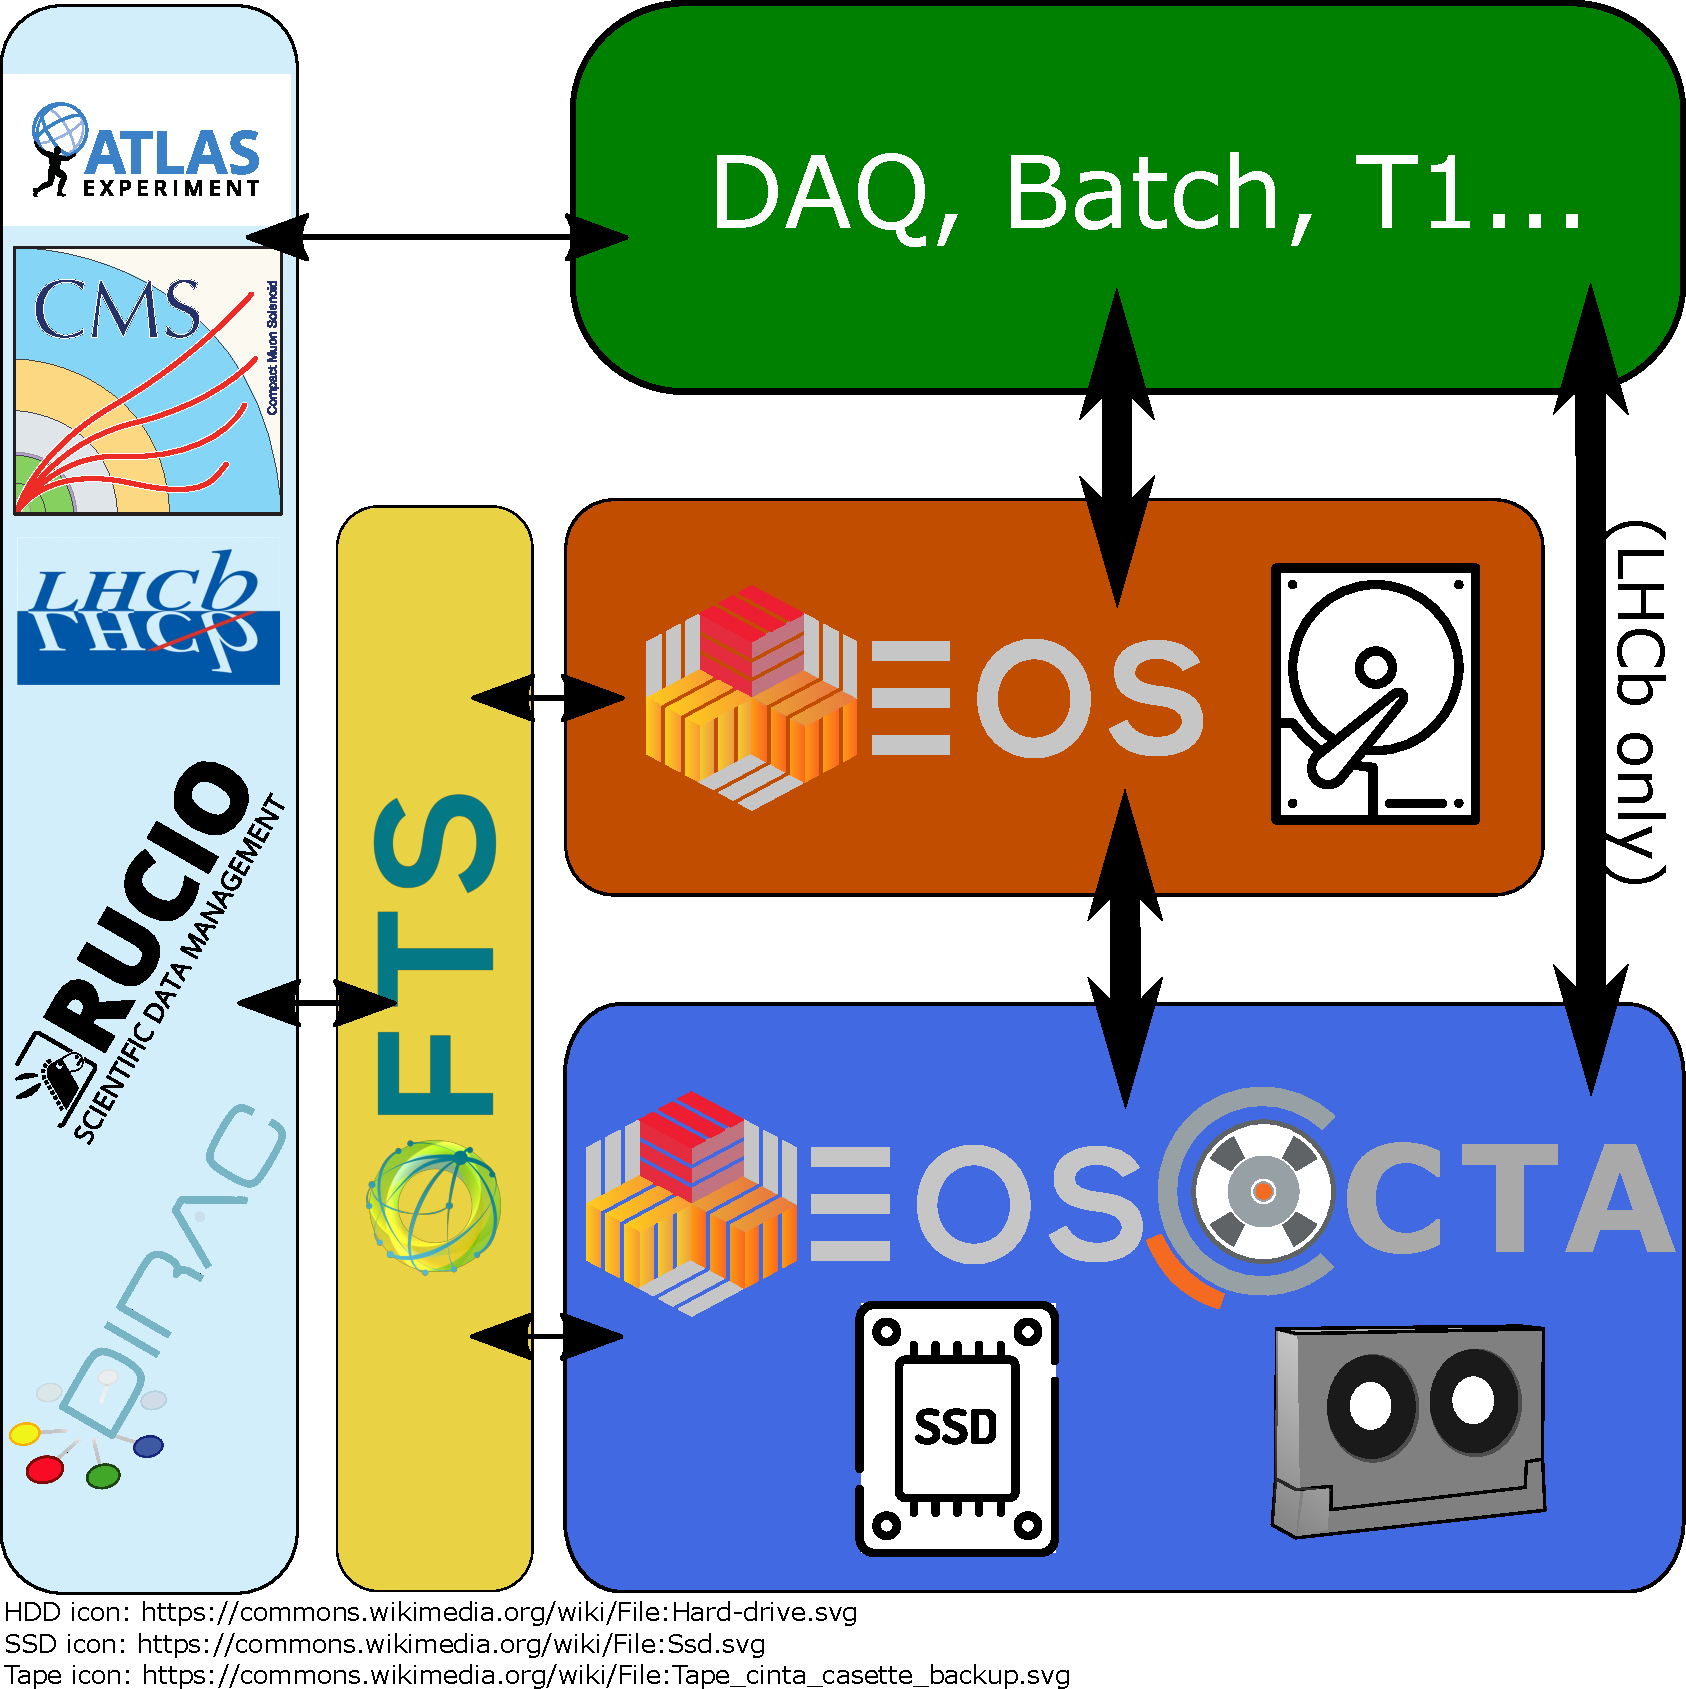
\includegraphics[width=\linewidth]{images/withNewLogo/CTA_Deployment_Atlas_CMS_LHCb}
   \caption{General model of CTA deployment, as followed by ATLAS, CMS and LHCb}
   \label{fig:general_deployment}
\end{wrapfigure}

CTA is a pure tape backend~\citep{cta_chep2016},~\cite{cta_chep2018} providing a tape storage tier to EOS instances.
A single CTA instance serves multiple EOS instances. This allows sharing the tape infrastructure
between various EOS front ends. During the rest of this article, we will refer to such EOS instances fronting CTA as
EOSCTA instances.

The EOSCTA instances are focused on buffering data coming in and out of tape. This buffering is achieved with SSD based
EOS disk spaces. SSDs deliver a well defined bandwidth, without non-linear degradation under load (disk thrashing,
as experienced by HDDs).

This guaranteed bandwidth comes at the price of a reduced size buffer. As a consequence, the files transferred to and from
tape cannot be kept for a long time in the disk buffer of the EOSCTA instance. When writing to tape, EOSCTA automatically
evicts the disk copy from the buffer. When reading from tape, this eviction should be done explicitly by the user. A garbage
collector completes the coverage to free the buffer of any files left behind.

In the typical deployment scenario, the destination of the file is the main EOS instance for the experiment. Those EOS instances,
targeting physics analysis, are based on HDDs to deliver a large volume of data. In data retrieval, the sequence of issuing a prepare request,
waiting for the file to be available in the EOSCTA buffer, triggering and following up the EOSCTA to EOS third party copy
and finally evicting the file explicitly from the buffer can be managed by the File Transfer Service (FTS)~\cite{fts_chep2019}. Data acquisition is
also encouraged to go through the main EOS instance and then to handle the transfer to EOSCTA and tape and its monitoring
via FTS. This layout is represented in figure~\ref{fig:general_deployment}.
% ITTF: https://indico.cern.ch/event/843592/

\subsection{Current infrastructure}
%\subsubsection{Infrastructure}

% Numbers from ITUM 29 presentation: https://indico.cern.ch/event/862894/contributions/3719964/attachments/1988270/3313847/CTA_Deployment.pdf
The currently deployed hardware for the EOS parts of the EOSCTA instances runs on 32 {\em{}hyperconverged} servers.
Each contains $16\times\SI{2}{\tera\byte}$ SSD drives. The servers are connected to the backbone via 
$6\times\SI{100}{\giga\bit\per\second}$ network links. Each server has a $\SI{25}{\giga\bit}$ Ethernet interface. 
Currently, 29 tape servers complete the setup. Tape servers can be re-installed to run either CASTOR or CTA, so the
number of drives can be adjusted as necessary during the transition from CASTOR to CTA. The servers are called
{\em{}hyperconverged} as they fulfil all the tasks in an EOS cluster in a shared manner.
The SSDs serving the experiments are interleaved in the various servers, along with the ones containing the
metadata database of EOS: quarkDB. 
%The detailed architecture of an EOSCTA system and its environment will be discussed in
%section~\ref{sec:integration}.


\subsection{Integration with EOS and FTS}
\label{sec:integration}

%\subsubsection{Tape operations through EOS}

In the EOSCTA system, the EOS instance handles all the name space operations. Only operations involving the
tape system are forwarded to CTA by EOS. Those operations include validation of file creation,
triggering archiving and retrieving from disk to tape and {\em{}vice-versa}, as well check upon
file creation, file deletions and cancellation of retrieves.
%\subsubsection{CTA notification to EOS and FTS}

CTA reports the result of archive and retrieve operations to the user via EOS and optionally FTS.
Upon successful write to tape, EOS also automatically deletes the disk copy from cache.
When using FTS, the file is further transferred out of EOS to its destination and the copy in the 
cache is evicted. FTS also retries in case of failed operations.

%\subsubsection{Activities fair share}
An activities mechanism, where FTS allows users to give weighted shares of bandwidth to activities competing
for tape bandwidth within the same VO, has been implemented in CTA as well. This feature allows FTS to forward
the activity information for retrieves and gives each activity a share of tape mounts proportional to its weight.

%\subsubsection{Cache management and garbage collection}
\subsection{Disk space management}

All pure disk cache operations are handled locally by EOS. Those include
all metadata queries, file access by the user, and disk cache management. The latter provides 
both explicit cache eviction, and garbage collection. These new features were added to xrootd and EOS.

%\subsubsection{Back pressure}
%\label{subsubsec:backpressure}

The disk cache on SSDs is dimensioned to hold 8 hours of traffic.
Several mechanisms were developed to protect it. A back pressure
mechanism was created for retrieves from CTA to EOS, where the tape system keeps a tally of the sizes of the files
to be written from tape to disk and does not commit to operations that would eventually overflow.

Likewise, a back pressure mechanism is under development in FTS and EOS where EOS will provide the available space
in the disk cache to FTS, which will back off before overflowing the buffer. Currently, FTS experiences failed transfers
due to overflow and retries, which wastes bandwidth.

\section{Integration with experiments work flows and results}
\subsection{ATLAS}
%\subsubsection{Deployment model}

The ATLAS experiment got involved early for the integration of its data management system, Rucio~\cite{rucio}, with CTA.
This integration follows the general deployment model for CTA, where Rucio delegates the transfers to FTS. 
The layout is represented on figure~\ref{fig:general_deployment}.

%\subsubsection{Results}
% Production hardware as a reference
% 2x Intel Xeon Scalable 5218 processors
% 192GB of DDR4 ECC Reg memory running at 2667 MHz (M393A2K43BB1-CTD)
% 1x 512GB Samsung 970 EVO Plus NVMe SSD for OS (MZ-V7P512BW)
% 16x 1.92TB Intel S4510 SSD (SSDSC2KB019T801) running firmware >= XCV10110 (~500MB/s per SSD of read+write throughput)
% 2x 25Gbit/s Ethernet ports (one used)
ATLAS workflows have been heavily exercised on the various hardware deployments of the CTA preproduction infrastructure.
Its latest incarnation is running on the final production hardware and served the Atlas data17 reprocessing share for T0.

In this context, 800TB were recalled, 317078 files of 2.5GB each, with 350 failures whose causes are understood.

The average read rate was 4.6 GB/s when there were enough queued requests. Enterprise tape drives were reading tapes with RAO at rates between 250 and 280 MB/s on average (~80\% of max drive speed).

The service scaled smoothy as more hardware was added to it: with those tests we showed that the performance could be scaled while maximising buffer and tape drive efficiency.

\subsection{CMS}

The CMS experiment is planning to migrate its data management to Rucio, following the model of ATLAS.
The deployment is still ongoing. This is represented in figure~\ref{fig:general_deployment}.

\begin{wrapfigure}{R}{0.45\textwidth}
   \includegraphics[width=\linewidth]{images/withNewLogo/CTA_Deployment_ALICE}
   \caption{CTA deployment model for the ALICE experiment with SSD and HDD storage tiers for the EOSCTA cache}
   \label{fig:ALICE_deployment}
\end{wrapfigure}

\subsection{LHCb}

The LHCb experiment is also planning a similar deployment, using Dirac as the data and workload management framework~\cite{dirac}.
Occasional direct exports
to tier 1 storage elements will happen, slightly circumventing the general model. As this out of model traffic
is expected to be low, the extra space required by the higher latency transfers over the Grid is expected
to be small enough to fit in the SSD based storage. This deployment is shown in figure~\ref{fig:general_deployment}.

\subsection{ALICE}

The deployment of ALICE will be the most divergent from the general model. ALICE does not use
FTS and will not be able to release disk cache after retrieves. Two-step retrieve (from tape to
EOSCTA disk cache to EOS) will also not be possible. For these reasons, the EOSCTA instance will
have two spaces, one with SSDs and one with HDDs. Archives will go through SSDs as in other cases,
while retrieves from tape will go to HDD via the SSDs to ensure optimal tape drive bandwidth. 
The garbage collector will free up the HDD, without external management from the
experiment. This layout is represented in figure~\ref{fig:ALICE_deployment}.

\section{Newly implemented and planned features to the software stack}
%
%\subsection{New features to CTA}
%  \begin{itemize}
%    \def\fnm1{\footnotemark[1]}
%    \item Tape server: Tape alert support, HW RAO (enterprise drives), SW RAO (LTO)\footnote[1]{Explained in backup slides},
%    LBP, encryption, empty file skip on write\fnm1.
%    \newline{}
%    \item Scheduler: Priorities, drive dedication, fair share between VOs\fnm1, intra-VO weighted fair share (activites)\fnm1,
%       mount pre-emption\fnm1, backpressure\fnm1, dataset colocation\fnm1, repack request expansion on demand\fnm1
%    \item EOS: Garbage collection, retrieve request filtering, retrieve request cancellation, disk copy eviction
%    \item FTS: Multi hop, eviction after transfer.
%  \end{itemize}

In addition to the features involving the interface between CTA, EOS and FTS, already mentioned
in section~\ref{sec:integration}, several features expanding the CTA scheduling have been developed or planned.
New tape labelling support was also added.

\subsection{Repack}
Repack functionality was added to CTA. Although not user visible, repack ensures 
data safety by moving it out of failing tapes and into new ones. 
Repack also allows migration to new media generations over time.

Repack incorporates new features, previously managed by external scripts.
A feed mechanism allows programming the repacking of many tapes without overflowing the
scheduling system with just in time expansion of tape entries into all their individual files.
Operators can also preload the data for files has been manual extracted from failing tapes.

\subsection{Back pressure}
In order to protect the disk cache from overflow, an optional back pressure mechanism has been put in place,
where the tape drives will globally register writes, reserving space and ensuring that they do not globally
exceed an operator defined free space threshold during retrieves.

\subsection{Tape labeling}
IHEP (Protvino, Russia) contributed a tape labelling utility, ported from CASTOR. This command line tool for operators 
provides the same level of validation and safety for this potentially destructive operation by making sure that no file
on the tape being labelled is referenced in CTA.

\subsection{FIFO mounting and Queue performance optimization}
At the request of experiments, the scheduling of tapes for retrieve is FIFO based: with equal priority,
the tape with the older retrieve request will be processed.

The object store used to queue the requests to CTA has been further optimized, reaching $\SI{200}{\hertz}$ per queue.
This improvement reduces bandwidth degradation in small files scenarios where metadata operations become the limiting factor.


%\subsection{Planned features}

\subsection{Colocation hints/smart writing (planned)}
Multiple experiments are requesting smart writing. This feature will
allow them to tag files by dataset. With this information, the tape system will store related files
together. This will lead to optimal read performance, with no positioning between
files when reading a full dataset, as experiments do most of the time.

This is a better alternative to creating huge files. $\mathcal{O}(\SI{100}{\giga\byte})$
sizes were discussed. Such files would exceed the size of the system memory of the tape
servers, and prevent having multiple disk transfers in parallel. Multiple disk streams are needed to attain the full 
tape bandwidth (roadmaps for tape drives plan for $\SI{1}{\giga\byte\per\second}$ in the medium term).

\subsection{RAO on LTO (planned)}
In the absence of smart writing, achieving good read performance when only a small fraction of a tape is being read requires
carefully choosing the order of the files being read, taking into account their positions
on the $\mathcal{O}(100)$ wraps holding the data on the tape.

Enterprise tape drives provide a recommended access order (RAO) query mechanism, which CTA uses, to
determine this optimal order. The performance gains are significant~\cite{cristina_msc_thesis}.

Linear Tape Open (LTO)~\cite{LTO} tape equipment it an alternative to enterprise-class. 
Unfortunately, LTO drives do not provide this RAO mechanism. Without it, a higher amount of time is spent in seeks,
bringing down the retrieve performance.

A proof of concept of a software based RAO, computed from outside the drive, has been validated~\cite{German_LTO_RAO}.
This mechanism needs to be developed further, and will require CTA to store in its file catalogue the values or estimates of
the physical position of the files on tape.

\subsection{Preemptive scheduling (planned)}
In order to efficiently use the tape drives, a preemptive scheduling is planned where low priority mounts
will use the hardware as much as possible, freeing it up mid-mount if a higher priority mount
appears. Currently a tape drive will not be freed up before the mount is complete. This feature would 
replace external scripts used in CASTOR and reduce the latency seen by higher priority mounts while 
maximising the hardware usage.

\section{Multiple database backends}


%This section gives a brief description of the multiple database ends supported
%by CTA, discusses some of the more interesting developments that were made
%during 2019 and explains how the Oracle database backend was used in production with
%the ATLAS experiment.

CTA has a central relational-database that catalogues the locations of all the
files that have been archived on tape (the CTA catalogue).

The CTA catalogue provides support for multiple backends in production:  
MariaDB, Oracle and PostgreSQL. CTA also uses an in-memory SQLite database
backend for unit tests. All backends are equally validated in continuous
integration since September 2019, ensuring the absence of regression bugs.

The Oracle database backend will be used at CERN for the first production
deployment of CTA, as recommended by the CERN database group given the 
availability and data recovery requirements requested by the CTA team.

CERN ultimately plans to migrate the CTA catalogue from Oracle to PostgreSQL.
Running CTA on an open source database will reduce licensing costs. 
External sites interested in using CTA have also
indicated their preference to use open source database solutions.
The design and implementation of the CTA catalogue minimized the use 
of vendor specific features to allow multiple backends and hence avoid vendor lock in.
To this end CTA does not use Oracle PL/SQL unlike its predecessor CASTOR.

During 2019 the Rutherford Appleton Laboratory, UK made the decision to
gradually replace their existing CASTOR installation with EOSCTA. In this
regard they will follow CERN in their choice of database backend. They will
initially use Oracle and then migrate to PostgreSQL.

The Institute of High Energy Physics, Beijing, China (IHEP) has implemented the
MariaDB backend for the CTA catalogue.  IHEP wanted an open source solution and
have a considerable amount of experience with running MySQL databases.

The CTA catalogue has been put to test successfully in production during the ATLAS
reprocessing campaigns. It was pushed up to 60 million files with no sign
of performance issue.

\section{Migration from CASTOR to CTA}

The CTA Tape Server is an evolution from the CASTOR Tape Server and the underlying data format of files on tape is exactly the same.
This means that migration from CASTOR to EOSCTA is a pure metadata operation without physical data movement. The CASTOR namespace 
(directory/file listing) and tape catalogue will be imported to EOSCTA, and the tapes ownership will 
be handed over from CASTOR to EOSCTA. Prior to a migration operation, the corresponding namespace area will be frozen in CASTOR. Likewise, 
tapes imported from CASTOR are immutable in CTA. This will give the option of handing back the tapes to CASTOR and roll back the operation.

Importing into EOSCTA actually requires two distinct operations: injection of the tape file information in the CTA catalogue,
and injection of the directory and file structure into the EOS namespace of the buffer. Files in EOS reference the
tape files from the CTA catalogue.

As CASTOR is a system with both disk and tape elements, not all files will be migrated to CTA. Specifically, files with no
tape copy will not be migrated, nor will files which have been deleted but still exist in the CASTOR Tape Catalogue.
In addition, a decision was taken to simplify CASTOR metadata on import. CASTOR's legacy ACLs will be dropped, along with
the special POSIX bits---\texttt{S\_UID}, \texttt{S\_GID}, \texttt{S\_VTX} (sticky bit) as they cannot 
be mapped in the permissions in EOS. Symbolic links will also not be migrated.

CASTOR has a single namespace instance for all VOs. It was decided to use the migration as an opportunity to split the namespace
into instances aligned with the EOS disk (ATLAS, ALICE, CMS, LHCb and public).

Dry-run migration from CASTOR to CTA gave the opportunity to identify and cleanup a few corner cases: some 
tape pools contained files from multiple VOs, which were separated by repacking them to more appropriate tape pools.

The ATLAS migration has been carried out several times in 2019 and 2020, to give a complete snapshot of the ATLAS data in CTA,
which was then used for the ATLAS Run--2 data reconstruction campaign.

It is planned that the live migration of the tapes from the four LHC experiments will be completed during 2020 in order to start Run--3
data taking on CTA.

\section{Conclusions}

CTA has seen many improvements during 2019 and early 2020 which have allowed it to be used in production for the first time.  The ATLAS reprocessing campaign was a success and a very good test of CTA functionality, performance and stability.
The four LHC experiments are planned to be migrated from CASTOR to CTA before the start of Run--3.

The process of migration from CASTOR to CTA was validated. Multiple DB backends were implemented to ensure adequate solutions are available for deployment in different institutes. 

New features are in the development pipeline such as the software Recommended Access Order for LTO drives, preemptive scheduling and smart writing. These evolutions will improve CTA performance in order to fulfil the storage requirements of the LHC experiments for the coming years.

%
% ---- Bibliography ----
%
\bibliography{CHEP2019_CTA}

\end{document}
